\section{SCL engineering parts} 
\label{sec:SCL-engineering-parts}
The SCL description capability are 
an important \gls{SAS} engineering part, and may
start either with the SAS functional specification, 
\gls{IED} capability description or with the 
\gls{SAS} description. Theses steps 
are explained 
in the following subsections: 

\subsection{SAS functional specification}
The functional specification input to \gls{SAS} engineering 
consist in the system specification in terms of 
single line diagram, allocation of the \glspl{LN} 
and equipmets of the single line.

\subsection{IED capability description}
Another right name for this step is IED pre-engineering. 
In this step are described the IED capabilityes, for 
example, a IED with the double busbar line feeder function.

\subsection{SAS description}
\label{sec:SAS-description-scl-engineering}
This is part of the \gls{SAS} engineering, where the 
complete process configuration takes place: All IED 
are bounded to individual process functions and primary 
equipments, enhanced by access point connections and 
the access path in subnetworks for the clients.

A complete \gls{SAS} description provides 
all predefined associations and client-server connections 
(the \gls{IED} cannot built it automatically).

\todo[inline]{ver como puedo ir concatenando las ideas, hasta
desenvocar en este diagrama de secuencia}
A more detailed description are provided by this UML secuence diagram.

\begin{figure}
  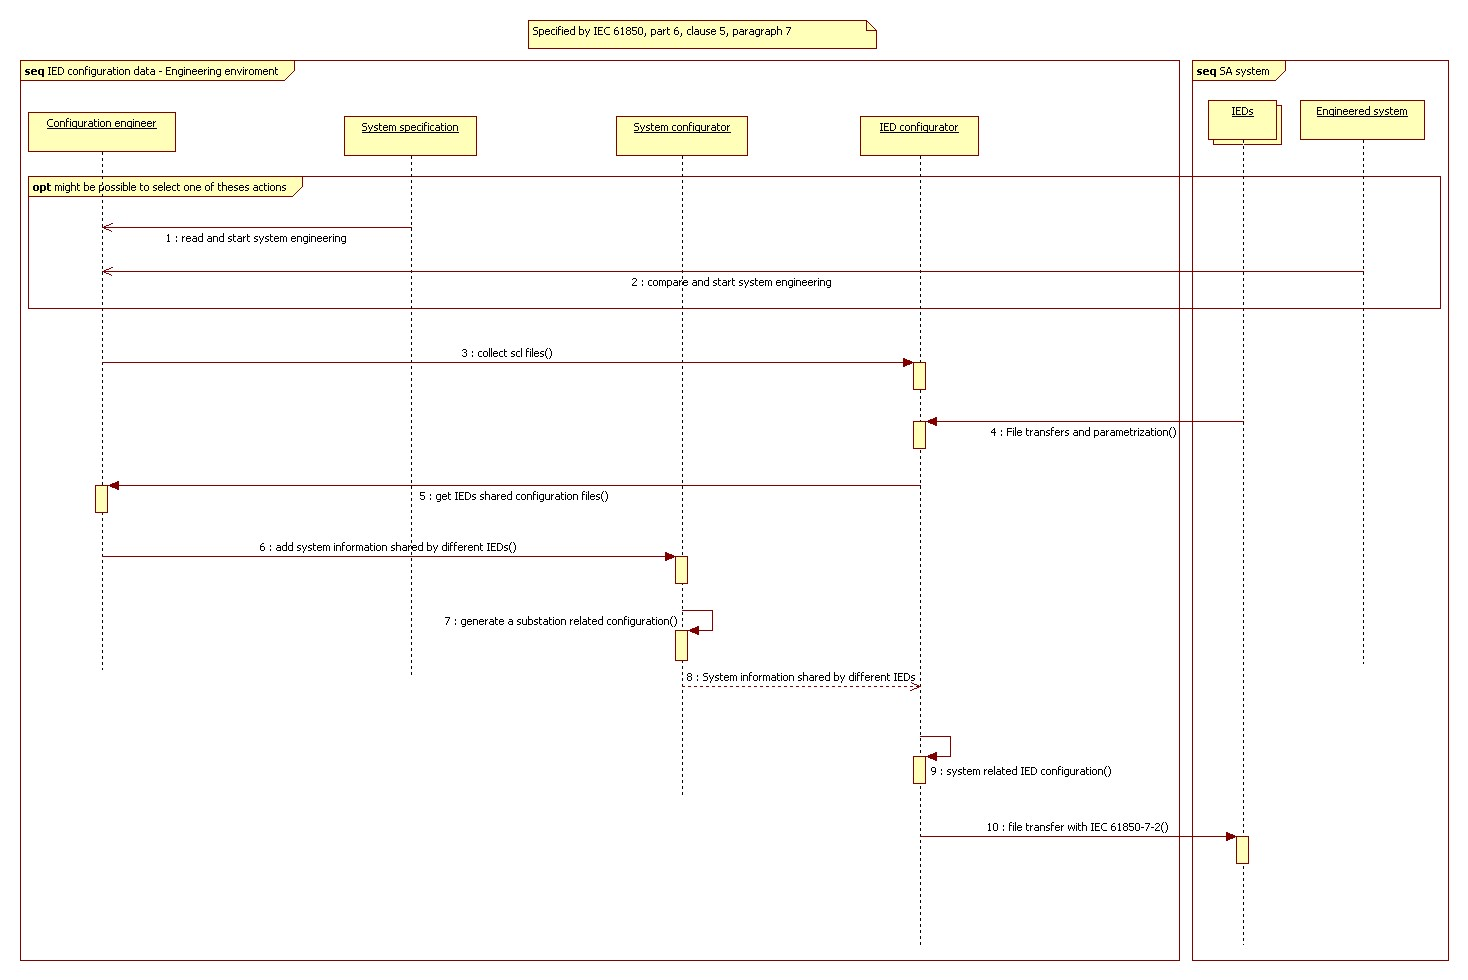
\includegraphics[width=1.0\textwidth]{chapters/ch-scl/figures/SCL-development-process}
  \caption{SCL engineering process}
  \label{fig:SCL-development-process}
\end{figure}

